\chapter{Robust Record-Level Web Extraction Algorithm}
\label{ch:algorithm}
% Describe your own work (how you reached your goal) and take care to motivate your choices. Don't just describe all the things you did – tell us why.

In this chapter, we introduce our algorithm for a robust record-level data extraction. We explain the main concepts and describe the logic in detail.


% ---------------
\section{Overview}

Given an initial web page snapshot with a single annotated book title, the algorithm extracts multiple movie titles from a future version of the same web page. The algorithm is designed to be fast and robust, requires only a single annotated page for training, and extracts data from multiple records inside a tree.

To illustrate the principles, we use a deliberately simple example from Figure~\ref{fig:amazon-books-html} and extract book titles from a web page. The main steps are depicted in Figure~\ref{fig:algorithm}.

\begin{figure}[h]
	\centering
	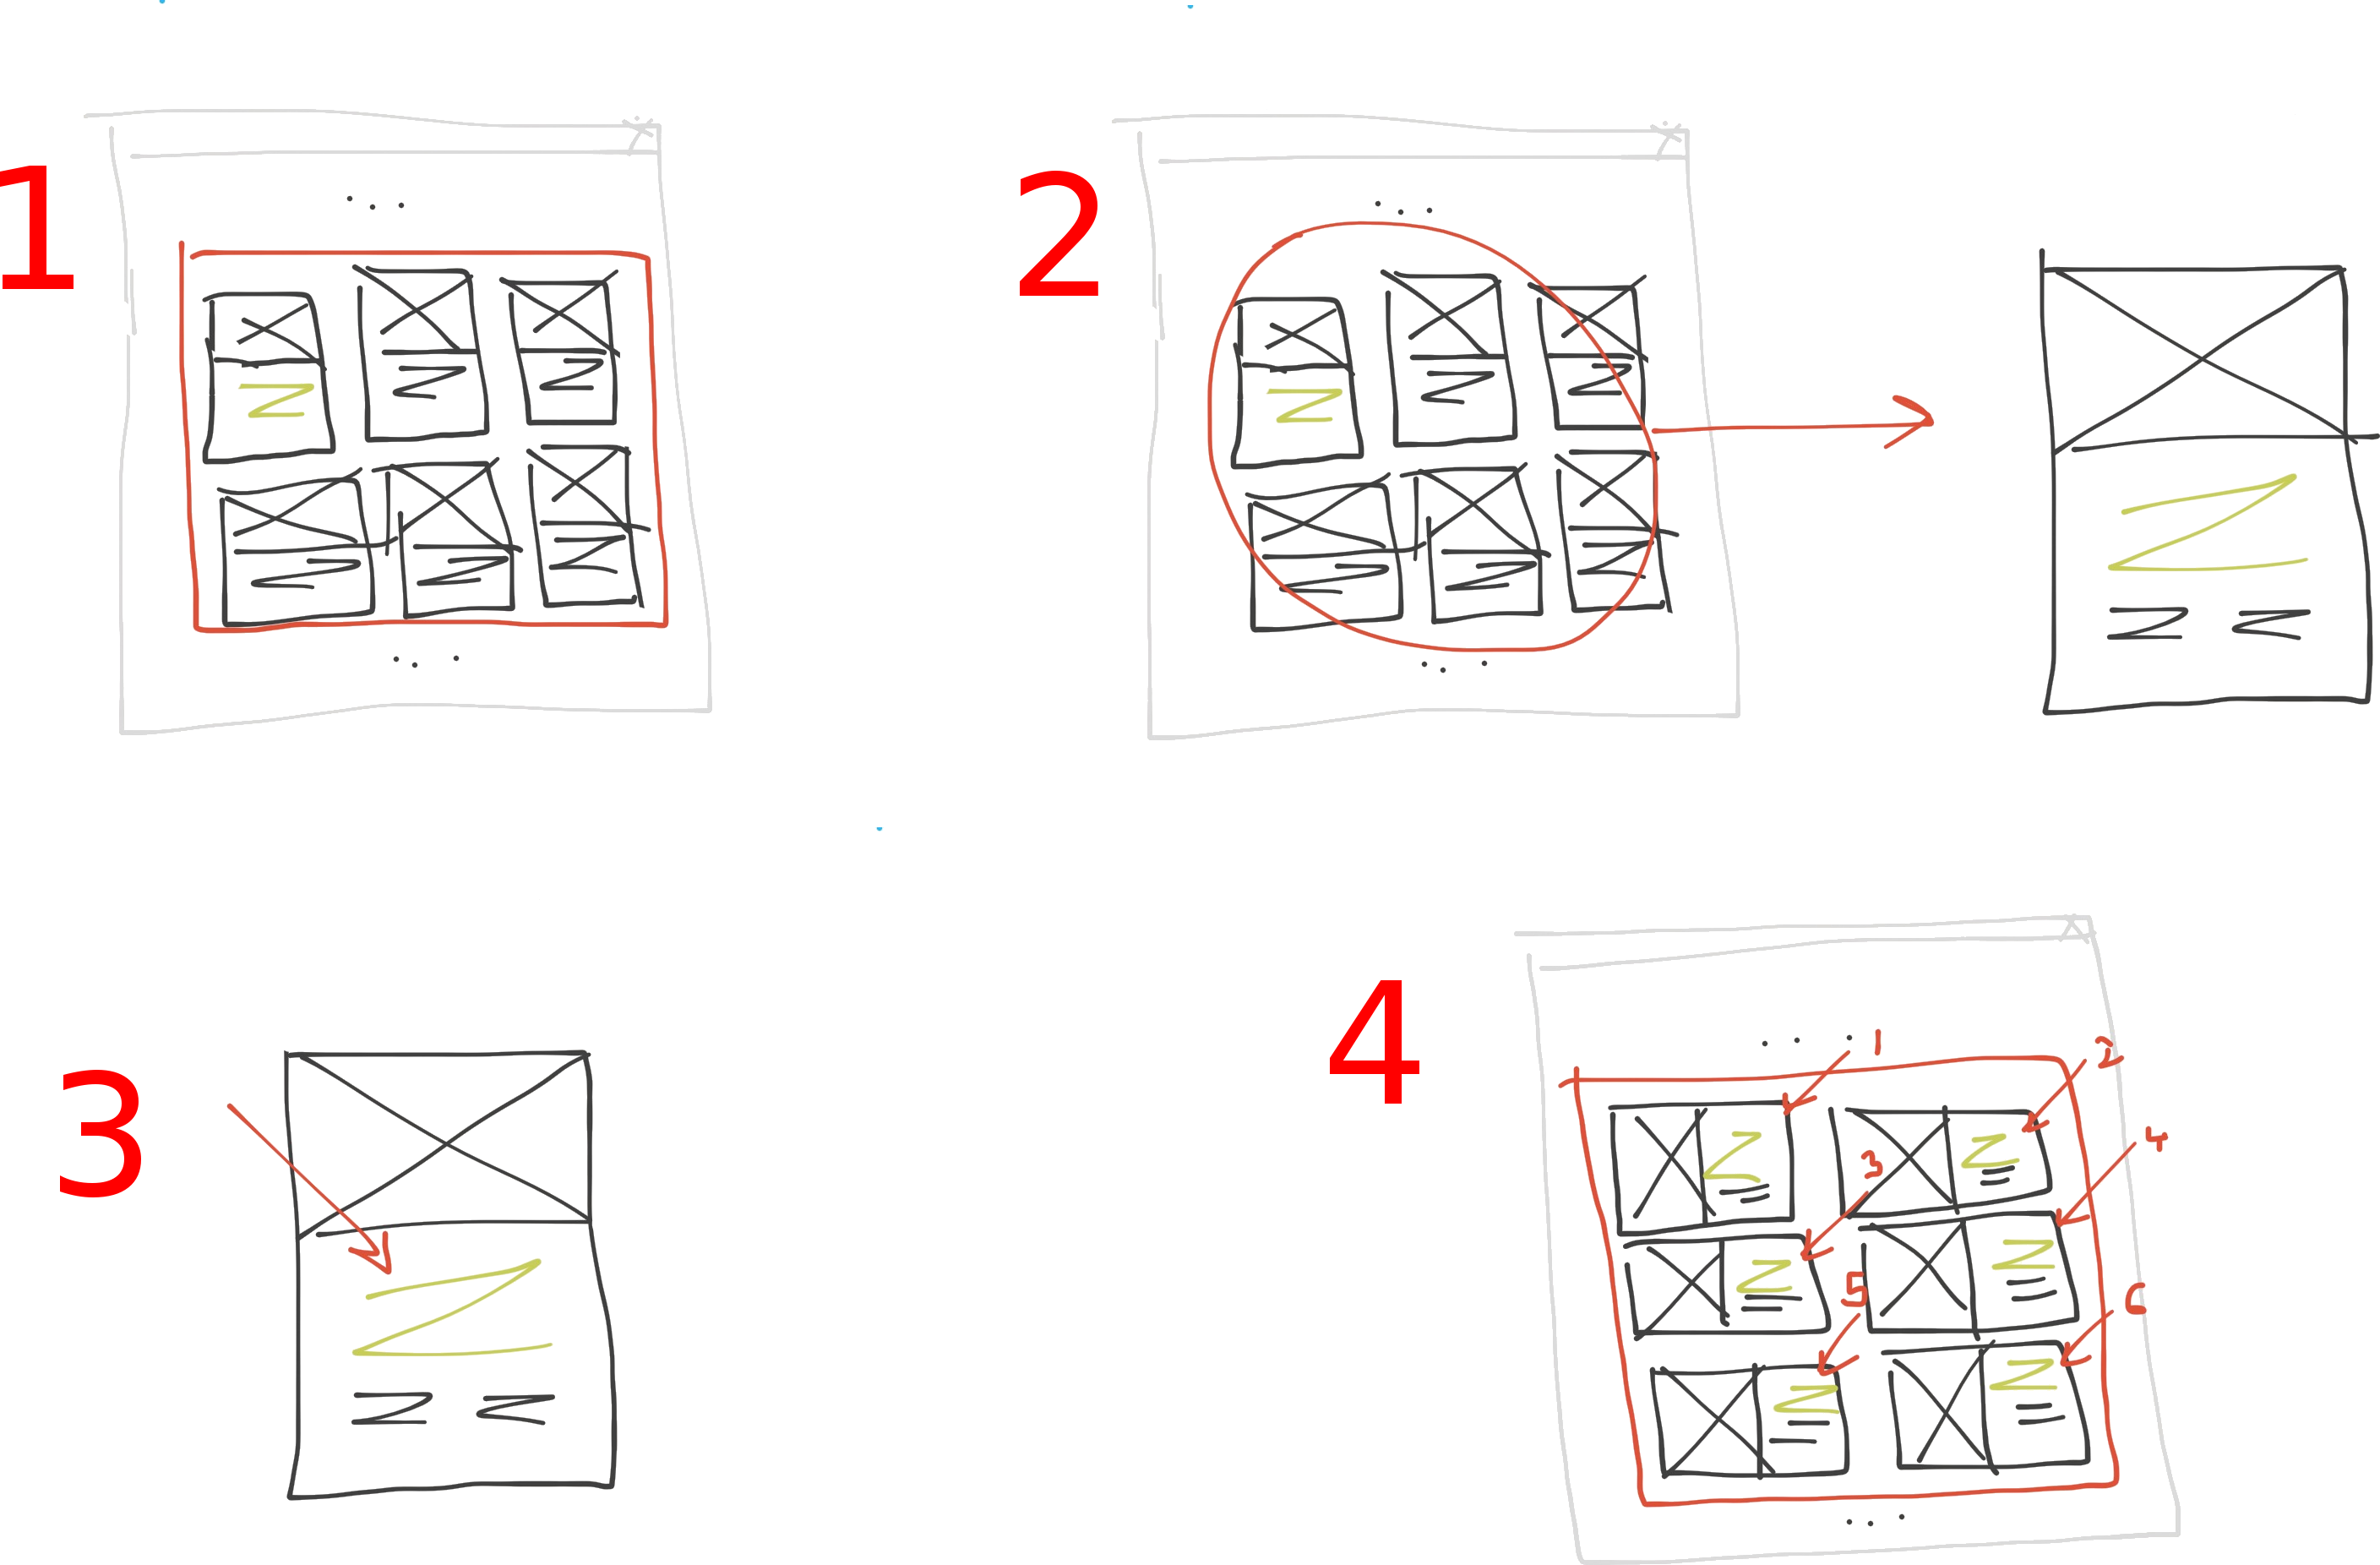
\includegraphics[width=1.0\textwidth]{figures/algorithm}
	\caption{Visualization of record-level wrapping steps.}
	\label{fig:algorithm}
\end{figure}

% How each method work. How they are combined.
The main idea of the new method is to split the wrapping process into two steps. First, we locate a relevant data region and find the boundaries of each data record. To cover structural variations, we progressively merge data records inside the original HTML into a generic tree. This tree is later used as a base for wrapping from the future pages. 

Next, we operate inside the boundary of each record in the transformed page and run a robust page-level wrapper. The wrapper is based on a tree-edit distance calculations with probabilistic HTML change model. The model captures how web pages evolve over time by looking at the likelihood of all possible changes \cite{dalvi2009a}.

% To illustrate the method in action..
The following example illustrates sample inputs and outputs. An initial snapshot $w_{base}$ of a sample HTML document is illustrated in Figure~\ref{fig:sample-tree}. The annotated attribute node $d(w_{base})$ is marked with parenthesis. The extracted record attribute values are $\{\text{Carol}, \text{Bob}, \text{Alice}\}$.
% TODO step-by-step with given example
% TODO Consider a transformed tree from Fig.~xx

\begin{figure}[h]
	\centering
	\Tree [.table 
			[.tr 
				[.td [.img ] ]
				[.td 
					[.a
						[.\textit{How to Build...} ]
					]
					[.a
						[.\textit{George...} ]
					]
					[.span 
						[.\textit{Hardcover} ]
					]
					[. ... ]
				]
			]
			[.tr 
				[. ... ]
			]
		]
	\caption{An initial $w_{base}$ (on the left) and a transformed $w_{new}$ (on the right) snapshots of a sample HTML document. Distinguished nodes marked in parentheses.}
	\label{fig:sample-tree}
\end{figure}


% ----------------------
\section{Core Algorithm}

% inputs, outputs, introduce notation and definitions
A detailed method for robust record-level wrapping is given in Algorithm~\ref{alg:prob-record-level-wrapper}. It operates on labeled, ordered, rooted tree structures. Thus, this is not limited to HTML documents only. The algorithm extracts a set of candidate nodes from a transformed tree, given the initial tree with a distinguished node. The inputs and outputs of the algorithm are described below.

Inputs: 

\begin{enumerate}
	\item $w$ -- an initial (labeled, ordered, rooted) tree with embedded data records.
	\item $d(w)$ -- a distinguished (usually textual) node within the initial tree, i.e. a single attribute node of a random data record.
	\item $w'$ -- a transformed tree.
\end{enumerate}

Outputs: 

\begin{enumerate}
	\item $\{c'_i\}$ -- A set of extracted candidate nodes in a transformed tree, i.e. single attribute values of all data records, e.g. book titles.
	%\item $c$ -- \emph{Confidence} measure, i.e. the probability measure that the wrapper did not break. This shows how accurate was the extraction.
\end{enumerate}

We assume that a distinguished node remains present in the future versions of the tree and is never deleted. The actual location of the node might change, though. For example, books listings web page in \url{amazon.com} will always contain book titles, even if the visual styling changes. This is a safe assumption, because a user annotates the DOM tree by pointing out the content of interest. And this is typically an important piece of information, that is preserved over future (HTML document) updates. Thus, there is a single distinguished node $d(w) = \pi(d(w))$ in the new tree $w'=\pi(w)$, i.e. the node that a distinguished node $d(w)$ is mapped to by applying transformations $\pi$.

\IncMargin{2em}
\begin{algorithm}[h]

	\SetKwFunction{LocateDataRegionContainingNode}{LocateDataRegionContainingNode}
	\SetKwFunction{MergeDataRecords}{MergeDataRecords}
	\SetKwFunction{ProbWrap}{ProbWrap}
	\SetKwFunction{FindRegionContainingNode}{FindRegionContainingNode}
	\DontPrintSemicolon

	\KwData{$w, w', d(w)$}
	\KwResult{$\{c'_i\}$}
	\BlankLine

	$dr$ = \LocateDataRegionContainingNode($w$, $d(w)$) \;
	$r$ = \MergeDataRecords($dr$) \;

	$c'$ = \ProbWrap($w$, $d(w)$, $w'$) \;
	$dr'$ = \LocateDataRegionContainingNode($w'$, $c'$) \;

	\Return $\left\{ \ProbWrap(r, d(w), r') \right\}$, $\forall r' \in dr'$ \;

	\caption{Probabilistic record-level wrapper.}
	\label{alg:prob-record-level-wrapper}

\end{algorithm}
\DecMargin{2em}

% line-by-line how it works
The Algorithm~\ref{alg:prob-record-level-wrapper} first locates the data region $dr$ in the original tree $w$ that contains the distinguished node $d(w)$ as in Line 1. In Line 2, the data records from the data region $dr$ are merged into a generalized record $r$. As tree structure might slightly vary per record, this step ensures that the base record for wrapping contains the most general template. The candidate node $c'$ is identified on Line 3. With that, on Line 4 a data region $dr'$ in the transformed tree $w'$ is located. Finally, each data record $r'$ from the newly found data region $w'$ is locally wrapped with a probabilistic wrapper on Line 5.

% Edge cases
Edge cases, like "the web page that has no data records" or "no candidate node has been found", have been omitted for simplicity reasons. In the first case, we could simply run page-level wrapper instead. In the second, we could terminate and throw an error. 

% Correctness
Wrapping accuracy in our algorithm relies on (1) how well data records are identified and (2) how accurate probabilistic wrapper performs per each record. While \texttt{ProbWrap()} returns provably optimal candidate \cite{DBLP:journals/pvldb/ParameswaranDGR11}, data region locator has somewhat weak definition of correctness. Therefore, we rely on empirical evidence (see Chapter~\ref{ch:results}) for accuracy evaluation.

% The building blocks and motivation
The Algorithm~\ref{alg:prob-record-level-wrapper} consists of three main methods, which are described in the following sections:
\begin{description}
	\item[LocateDataRegionContainingNode] which recognizes template generated areas in a tree.
	\item[MergeDataRecords] which aligns trees into a generalized template.
	\item[ProbWrap] which extracts data from a single data record in a robust way.
\end{description}

% Time complexity
\paragraph{Time complexity} The execution of Algorithm~\ref{alg:prob-record-level-wrapper} is linear. Thus, its time complexity equals the complexity of its most complex member function (see sections below for discussion on complexity of each). The execution of \texttt{LocateDataRegionContainingNode} is the slowest component; it has the complexity of $O(n_1 n_2^2 d_1)$, where $n_1$ and $n_2$ are the sizes of trees and $d_1$ is the depth of the first tree. We execute this method for each data record. This gives the total time complexity of our algorithm of $O(n_1 n_2^2 d_1 m)$


% --------------------------------------------
\section{Locating Data Region Containing Node}

% Why? Alternatives? 
To enable wrapping in a web page with multiple data records, we need to locate individual data regions and run page-level wrapper inside a single record. For that matter, we have chosen Liu et al. \cite{liu2009a} proposed technique for data record mining. Unlike most alternatives \cite{buttler2001a} \cite{csie2009a} \cite{jiang2009a} \cite{lerman2004a}, this method supports both contiguous and noncontiguous data records and is reported to be more accurate.

% limitation
However, there are a few limitations to this method. As long as a page contains at least two data records, the algorithm will automatically find them. But it will not work on single-record pages. We can handle this edge case easily by running page-level wrapper inside the page. Moreover, the algorithm is optimized for finding records in \texttt{<FORM>}, \texttt{<TABLE>}, \texttt{<TR>}, \texttt{<TD>} tags, but not more generic \texttt{<DIV>} trees. But since majority of web records live in table tags, we accept this limitation.

% Inputs and outputs
Given a tree with embedded data records, the Algorithm~\ref{alg:locating-data-region-containing-node} locates a data region with a distinguished node. The inputs and outputs are described in detail below.

Inputs: 

\begin{enumerate}
	\item $w$ -- a (labeled, ordered, rooted) tree with embedded data records.
	\item $v$ -- a distinguished node from a tree $w$.
\end{enumerate}

Outputs: 

\begin{enumerate}
	\item $dr$ -- a data record from a tree $w$ that contains a distinguished node $v$.
\end{enumerate}

% algo definition itself
\IncMargin{2em}
\begin{algorithm}[h]

	\SetKwFunction{TreeContainsNode}{TreeContainsNode}
	\SetKwFunction{MDR}{MDR}
	\SetKwFunction{Trees}{Trees}
	\DontPrintSemicolon

	\KwData{$w$, $v$}
	\KwResult{$dr$}
	\BlankLine

	$\left\{dr_i\right\}$ = \MDR($w$) \;
	\ForEach{$dr_i \in \left\{dr_i\right\}$} {
		\ForEach{$t_j \in \Trees(dr_i)$} {
			\If{\TreeContainsNode($t_j$, $v$)}{
				\Return $dr_i$ \;
			}
		}
	}

	\caption{Locating data region containing node}
	\label{alg:locating-data-region-containing-node}

\end{algorithm}
\DecMargin{2em}

% Step-by-Step
The detailed description of the method for locating a data region with a node is given in Algorithm~\ref{alg:locating-data-region-containing-node}. First, we locate all data regions per tree in Line 1. We make a call to \emph{Mining Data Records} (MDR) algorithm as described in \cite{liu2009a}. This returns a set of all data regions found, not just the ones of interest. In lines 2-7 we iterate through all data records and trees inside those regions, to locate the data record of interest. Finally, we return a data record with a node of interest.

% Original MDR shortcomings
In MDR, Liu et al. \cite{liu2009a} use string edit-distance for comparing child subtrees. MDR traverses the tree from the root downward in a depth-first fashion. At each node, a  comparison of various combinations of the children subtrees is performed. While this method is efficient (runtime complexity of $O(|s_1||s_2|)$ for strings $s_1$ and $s_2$), it is not accurate for text intensive web pages. As an example, consider two paragraphs with different text inside. String-wise these two are very different, yet the tree structure is identical (\texttt{<P>} element has a single child element \texttt{TEXT}).

% Tree vs String edit distance
Generally, web pages have a tree structure and a fixed set of element labels. And there is semantics associated with hierarchy and naming of nodes in HTML. Therefore, by using string edit-distance for HTML we ignore much of the information that is embedded in structure. Moreover, tree-edit distance uses HTML change models from real world pages and takes into consideration which change is more common, i.e. probable. Whereas, string matching simply compares HTML letter by letter and loses valuable information.

% Updated MDR with tree edit-distance
Thus, we experimented with method variations by using tree-edit instead of original string-edit distance for tree matching. We have found the results to be more accurate in our experiments. But there is a penalty in time complexity. Indeed, compared to string edit-distance, tree edit-distance runtime complexity is magnitude higher, i.e. $O(n^3)$. In this case, we decided to prioritize precision over the execution time. Considering that data records are a small portion of the whole page, the actual difference in execution time was not significant.

% Edit-tree distance: RTED
For tree-edit distance calculations, we use RTED algorithm by Pawlik and Augsten \cite{pawlik2011a}. As discussed in Section~\ref{sec:tree-edit-distance}, their solution is efficient for all tree shapes and never runs in the worst case, if a better solution exists.

% Other params and optimizations
In order to improve performance, we experimented with a few parameters and heuristics. First, we set a limit on a number of maximum root nodes per data record. This greatly reduces the combinations space in MDR. We use a limit of max three nodes. Our experiments proved it to be a practical choice, which did not have impact on accuracy. Yet, for more exotic cases this number was left as a parameter in our algorithm.

Second, we experimented with various threshold values for edit-distance measure. We settled for $80\%$. This threshold is used in locating data regions and deciding, if the next fragment of tree belongs to the current data region. Again, this has been left as a parameter for future algorithm tuning.

Third, we only calculate tree-edit distance for trees that are not substantially different. As a rule of thumb, we consider two trees being substantially different only when they have node count difference above a threshold. This proved to reduce execution time dramatically without much effect on accuracy. We chose value of $66\%$ for this parameter.

% Complexity analysis O(N)
\paragraph{Time complexity} As the author of MDR shows, for a tree with $n$ nodes time complexity is $O(n K^2)$ times the complexity of edit distance calculation, which in our case is $O(n^3)$. $K$ is the threshold of max root nodes per data record. We have chosen 3. In total, this gives time complexity of $O(n^4 K^2)$. In fact, we rarely hit the upper bound, as our optimizations greatly reduce the search space.


% ----------------------------
\section{Merging Data Records}
\label{sec:merging-data-records}

% Why? Alternatives?
Data records tend to have slight variations inside a data region. For example, in a book listing, certain books have special prices, while other don't. In order to reconstruct a full data record template structure, we progressively align multiple data record trees and merge the differences into a single template tree. Having the most generic data record as an initial snapshot, allows to minimize the edit distance from other variants of data records. For example, this lowers the risk of mistakenly recognizing a book record with a special price as a too different from a book with only a regular price. 

% Inputs and outputs
Given a set of trees, the Algorithm~\ref{alg:merging-data-records} merges trees pairwise in a top-down order and returns a single merged template tree. Two trees are merged by subsequently aligning nodes layer-by-layer. At each step, if a node match is not found, then the algorithm attempts to expand the template tree by inserting the node into the template. The expanded template tree is then used in subsequent merging. Alignment takes into account only the structure of the tree, but not the data at the leaves. Input, output and algorithm details are provided below.

Inputs: 

\begin{enumerate}
	\item $\left\{t_i\right\}$ -- a set of trees.
\end{enumerate}

Outputs: 

\begin{enumerate}
	\item $tt$ -- a merged template tree.
\end{enumerate}


\IncMargin{2em}
\begin{algorithm}[h]

	\SetKwFunction{SimpleTreeMatch}{SimpleTreeMatch}
	\SetKwFunction{AlignTrees}{AlignTrees}
	\SetKwFunction{FindUnalignedNodes}{FindUnalignedNodes}
	\SetKwFunction{InsertIntoSeed}{InsertIntoSeed}
	\DontPrintSemicolon

	\KwData{$\left\{t_i\right\}$}
	\KwResult{$tt$}
	\BlankLine

	$tt$ = $t_0$ \;
	\ForEach{$t \in \left\{t_i\right\}$}{
		$m$ = \SimpleTreeMatch($tt$, $t$) \;
		$l$ = \AlignTrees($m$) \;
		$u$ = \FindUnalignedNodes($t$, $l$) \;
		$tt$ = \InsertIntoSeed($tt$, $u$) \;
	}
	\Return $tt$ \;

	\caption{Merging data records}
	\label{alg:merging-data-records}

\end{algorithm}
\DecMargin{2em}

% step-by-step
Line 1 initializes the template with the first tree. Line 2 iterates through each tree to be merged and merges template with each tree pairwise. Line 3 evaluates similarity of two trees by producing the maximum matching matrix $m$ through dynamic programming. Line 4 aligns the nodes from the two trees by tracing back in the matrix $m$. Line 5 locates the unaligned vertices $u$ from a tree $t$. These vertices are inserted into a template in Line 6.

% what's different from Zhai
The Algorithm~\ref{alg:merging-data-records} is a variation of \emph{PartialTreeAlignment} by Zhai \cite{zhai2005a} (see Section~\ref{sec:data-record-mining}). Methods \texttt{SimpleTreeMatch()}, \texttt{FindUnalignedNodes()}, \texttt{InsertIntoSeed()} and \texttt{AlignTrees()} are used from Zhai's work. An important distinction is the way these methods are composed. Unlike Zhai, we do not repeatedly try to match unaligned items with the template. We cannot allow any ambiguity in the template, as it would impose undesired differences between template and data records in future wrapping. For example, adding unaligned node at a wrong position in the template would add additional edit cost of removing the node between two trees in the first place.

% Complexity analysis O(N)
\paragraph{Time complexity} Having knowledge of a predefined template, Zhai and Liu \cite{zhai2005a} aligns two trees in $O(n_1 n_2)$ time ($n_1$ and $n_2$ are tree sizes). This does not require upfront pairwise matching as trees are matched only against the latest template (see Line 3). This leads to efficient dynamic programming solution, very similar to string matching. Lines 4-6 have linear or constant time complexity. We repeat simple tree matching for each data record. This gives the final complexity of $O(n_1 n_2 k)$, where $k$ is the number of data records that are being merged.


% ------------------------------
\section{Probabilistic Wrapping}

% Why? Alternatives? 
In the final step of the core Algorithm~\ref{alg:prob-record-level-wrapper}, a template tree is matched against new data records to locate the position of a distinguished node. We build on the work of Dalvi et al. \cite{dalvi2009a}, who introduce probabilistic HTML change model, and Parameswaran et al. \cite{DBLP:journals/pvldb/ParameswaranDGR11}, who use this model to find the most probable location of a node in a transformed tree. Most alternative wrapping techniques (see Sections~\ref{sec:wrapper-induction}~and~\ref{sec:html-aware-data-extraction}) require large training sets, or use no formal definition of robustness, and thus have weak confidence estimation.

% Inputs and outputs
Given an initial tree with a distinguished node, the Algorithm~\ref{alg:optimal-probabilistic-wrapper} locates the most probable candidate node in a transformed tree. This method calculates transformation probabilities for each candidate node and returns the one with the highest value. The procedure pre-calculates probabilities for subtrees, which makes iterating over the candidates less expensive.

Inputs: 

\begin{enumerate}
	\item $w$ -- an initial tree.
	\item $w'$ -- a transformed tree $w$.
	\item $u$ -- a distinguished node in initial tree $w$.
\end{enumerate}

Outputs: 

\begin{enumerate}
	\item $c$ -- the most probable location of a distinguished node $u$ in a transformed tree $w'$.
\end{enumerate}


\IncMargin{2em}
\begin{algorithm}

	\SetKwFunction{TP}{TP}
	\DontPrintSemicolon

	\KwData{$w, w', u$}
	\KwResult{$c$}
	\BlankLine

	\ForEach{$v \in w$}{
		$p_{1v}$ = \TP($P_1$, $P'_1$) \;
		$p_{2v}$ = \TP($P_2$, $P'_2$) \;
	}

	\ForEach{$t \subset w'$}{
		$p_{2v}$ = \TP($P_2$, $t$) \;
	}

	\ForEach{$v \in w'$}{
		\ForEach{$z \in P_2$}{
			$p_{2z}$ = \TP($P_{2v1z}$, $P'_{2v}$) \;
		}
		$p_{3v}$ = \TP($P_2$, $P'_2$) \;
		$Pr(v)$ = $p_{1v} \times p_{2v} \times p_{3v}$ \;
	}

	\Return $\operatorname*{arg\,max}_{v \in w} Pr(v)$ \;

	\caption{Optimal probabilistic wrapper.}
	\label{alg:optimal-probabilistic-wrapper}

\end{algorithm}
\DecMargin{2em}

In the description of Algorithm~\ref{alg:optimal-probabilistic-wrapper}, we split the tree $T$ into three parts and precompute probabilities separately. We use notation $T_v$ to note the tree under the node $v$. $P_1$ notes all nodes in the tree that are to its left from node $v$ or to the left of its ancestors in some tree $T$. $P_2$ notes the tree $T - T_v - P_1$. For details see Figure~\ref{fig:tree-parts}.

% Tree parts
\begin{figure}[h]
	\centering
	\includegraphics[width=0.5\textwidth]{figures/tree-parts}
	\caption{Tree parts.}
	\label{fig:tree-parts}
\end{figure}

% step-by-step
In the Algorithm~\ref{alg:optimal-probabilistic-wrapper}, the core function is \texttt{TP()}, which calculates the probability of transforming one tree to another \cite{dalvi2009a}. It uses a change model and tree-edit cost calculations to perform the task. Lines 1-4 pre-calculate probabilities of transforming prefix trees for all nodes. Lines 5-7 also pre-calculate probabilities, but for transforming $P_2$ to complete subtrees in $w'$. Lines 9-11 pre-calculate probabilities of prefix of $z$ in tree $P_2$ to tree $P'_2$. Final probability of transforming $P_2$ to $P'_2$ is calculated by Line 12. All of precalculated probabilities are multiplied in Line 13 to calculate the probability of $u$ being mapped to $v$. Finally, Line 15 returns the node $v$ with the highest probability.

% rewrite in own words
The method \texttt{TP()} calculates $P(\pi(w_1) = w_2)$, i.e. the probability of transforming a tree $w_1$ into a $w_2$, given a stochastic process $\pi$. As noted in Section~\ref{sec:tree-edit-distance}, $\pi$ performs insertion, deletion and substitution operations on ordered trees with predefined probabilities, i.e. a \emph{change model}. We use recursive definition of \texttt{TP()}, as described by Dalvi et al. \cite{dalvi2009a}. Here the probability of $\pi(F_s) = F_t$ is defined as a function $DP_1(F_s, F_t)$. The change model probabilities are notated with $P_{sub}()$, $P_{del}()$ and $P_{ins}()$. For edge cases and further discussion on recursive definition please refer to Section~4.1 in \cite{dalvi2009a}. 

\begin{equation}
	DP_1(F_s, F_t) = DP_2(F_s, F_t) + P_{ins}(v) \times DP_1(F_s, F_t - v)
\end{equation}

\begin{equation}
	\begin{split}
		DP_2(F_s, F_t) = P_{sub}(u, v) \times DP_1(F_2 - [u], F_t - [v]) \times DP_1(\lfloor u \rfloor, \lfloor v \rfloor) \\
		+ P_{del}(u) \times DP_2(F_s - u, F_t)
	\end{split}
\end{equation}

In order to optimize the performance of \texttt{TP()}, we have implemented a heuristic. We assume a probability of $w_1$ being transformed to $w_2$ as $0$, when two trees are substantially different. As in data region locator, we treat two trees as substantially different, if the count of nodes in both trees differs by more that $66\%$. This is a cheap operation in comparison to recursive calculations of \texttt{TP()}. As our experiment showed, this optimization has helped to reduce the execution time.

% Complexity analysis O(N)
\paragraph{Time complexity} Parameswaran et al. \cite{DBLP:journals/pvldb/ParameswaranDGR11} prove that page-level probabilistic wrapper (described in Algorithm~\ref{alg:optimal-probabilistic-wrapper}) has time complexity of $O(n_1 n_2^2 d_1)$, where $n_1$ and $n_2$ are node count per each tree and $d_1$ is depth of the first tree. 

Algorithm~\ref{alg:optimal-probabilistic-wrapper} is the slowest component in our algorithm. It is important to note, that we run it only per each data record, which is a tiny fragment of the whole tree. Practically, this should not hit to worst case time complexity and perform really fast.


% vim:wrap linebreak nolist:
